\documentclass[addpoints,11pt]{exam}

\usepackage{alltt}
\usepackage[margin=1in]{geometry}   % set up margins
\usepackage[T1]{fontenc}
\usepackage[usenames,dvipsnames]{xcolor}
\usepackage{enumerate}              % fancy enumerate
\usepackage{amsmath}                % used for \eqref{} in this document
\usepackage{amsthm}
\theoremstyle{definition}
\newtheorem{exmp}{Example}[section]
\usepackage{verbatim}               % useful for \begin{comment} and \end{comment}
\usepackage{eurosym}                % used for euro symbol
\usepackage{caption} 
\usepackage{graphicx}
\graphicspath{{Figures/}}
\usepackage{subcaption}
\usepackage{color}
\usepackage{float}
\usepackage{amssymb}
\usepackage{sgamevar}
\usepackage{sgame}
\usepackage[colorlinks=true]{hyperref}
\hypersetup{colorlinks=true, citecolor=ForestGreen, linkcolor=BlueViolet, urlcolor=Magenta}

%Solutions or nah (blank next two lines out for no solutions, unblank #3)
%\printanswers
%\newcommand{\dd}[1]{\par {\textbf{\textcolor{red}{#1}}}}
\newcommand{\dd}[1]{}  


\setlength\parindent{0pt}
\unframedsolutions
\SolutionEmphasis{\color{red}}
\CorrectChoiceEmphasis{\color{red}}
\renewcommand{\choicelabel}{(\alph{choice})}
\newcommand{\blank}[0]{\underline{\hspace{3cm}}}
\pointformat{\bfseries[\thepoints]}
\pointpoints{pt}{pts}
\pointsinrightmargin

\begin{document}
	
\title{\textbf{Final Exam} \\ \dd{Solutions\\} \vspace{2 mm} {\large ECON 101-002}}
\author{Summer I 2017}
\date{}
\maketitle

\makebox[\textwidth]{Name:\enspace\hrulefill}
\\

\makebox[\textwidth]{ONYEN:\enspace\hrulefill}
\\

\makebox[\textwidth]{PID:\enspace\hrulefill}
\\

\makebox[\textwidth]{Honor Code Signature:\enspace\hrulefill}
\\

Directions: Choose the option that best answers the question given. 

\subsection*{Economic Growth}

\begin{questions}

\question Which of the following is NOT a determinant of a country's long-run productivity?

\begin{choices} 
	\choice Human capital
	\CorrectChoice The money supply
	\choice Technological knowledge
	\choice Natural resources
\end{choices} 




\question Which of the following government policies is \textit{least} likely to increase economic growth?

\begin{choices}
	\CorrectChoice Increase restrictions on imported goods.
	\choice Increase expenditures on public education.
	\choice Reduce restrictions on foreign capital investment.
	\choice Eliminate widespread corruption.
\end{choices} 


	\question Which of the following would be considered an increase in human capital?

\begin{choices}
	\choice An increase in the use of heart disease centers.
	\choice The discovery of a cure for broken hearts.
	\choice An increase in the number of heart disease researchers.
	\CorrectChoice An increase in the training of heart disease researchers.
\end{choices}

\newpage

\question Productivity is defined as 

\begin{choices}
	\choice the stock of equipment and structures that are used to produce goods and services.
	\choice the inputs into the production of goods and services that are provided by nature.
	\choice the ``rules of the game'' that shape social interactions and structure economic incentives.
	\CorrectChoice the quantity of goods and services produced from each unit of labor input.
\end{choices}


\question A country has an annual growth rate of real GDP per capita of 2.5\%. Real GDP per capita in 2016 is \$20,000. Real GDP per capita in the country will be at least \$40,000 by

\begin{choices}
	\item 2040.
	\item 2030.
	\item 2035.
	\CorrectChoice 2045.
\end{choices}


\uplevel{\subsection*{Solow Model}}
	
	\question Consider Table \ref{tab1}. 
	
	\begin{table}[h!]
		\centering
		\caption{Production in Utopia}
		\label{tab1}
		\begin{tabular}{c|c|c|c|c|c}        
			
			$t$ & $k$ & $y$ & $i$ & $d$ & $\hat{y}$ \\
			\hline
			0 &  &  & $x$ & $y$ & ---\\
			1 &  & & &  & $.95\%$ \\
			2 &  & & & & $z$\\
		\end{tabular}
	\end{table}
	
	Under the assumptions of the Solow Model, which of the following is true?
	
	\begin{choices}
		\choice $x<y$ and $z>.95\%$
		\choice $x>y$ and $z>.95\%$
		\CorrectChoice $x>y$ and $z<.95\%$
		\choice $x<y$ and $z<.95\%$
	\end{choices}

\question A country's output per worker is described by the function $y=2\sqrt{k}$. Capital depreciates at a rate of 2\% and the labor force remains the same each period (i.e., $n =0$). If the country sets a savings rate of 30\%, what will be the level of \underline{output} per worker once the country reaches its steady state?

\begin{choices}
	\choice 900
	\choice 45
	\CorrectChoice 60 
	\choice 30
\end{choices}


\newpage



	\question Figure \ref{MC22} shows the identical production, investment and depreciation functions for countries $X$ and $Y$. 


\begin{figure}[H]
	\centering
	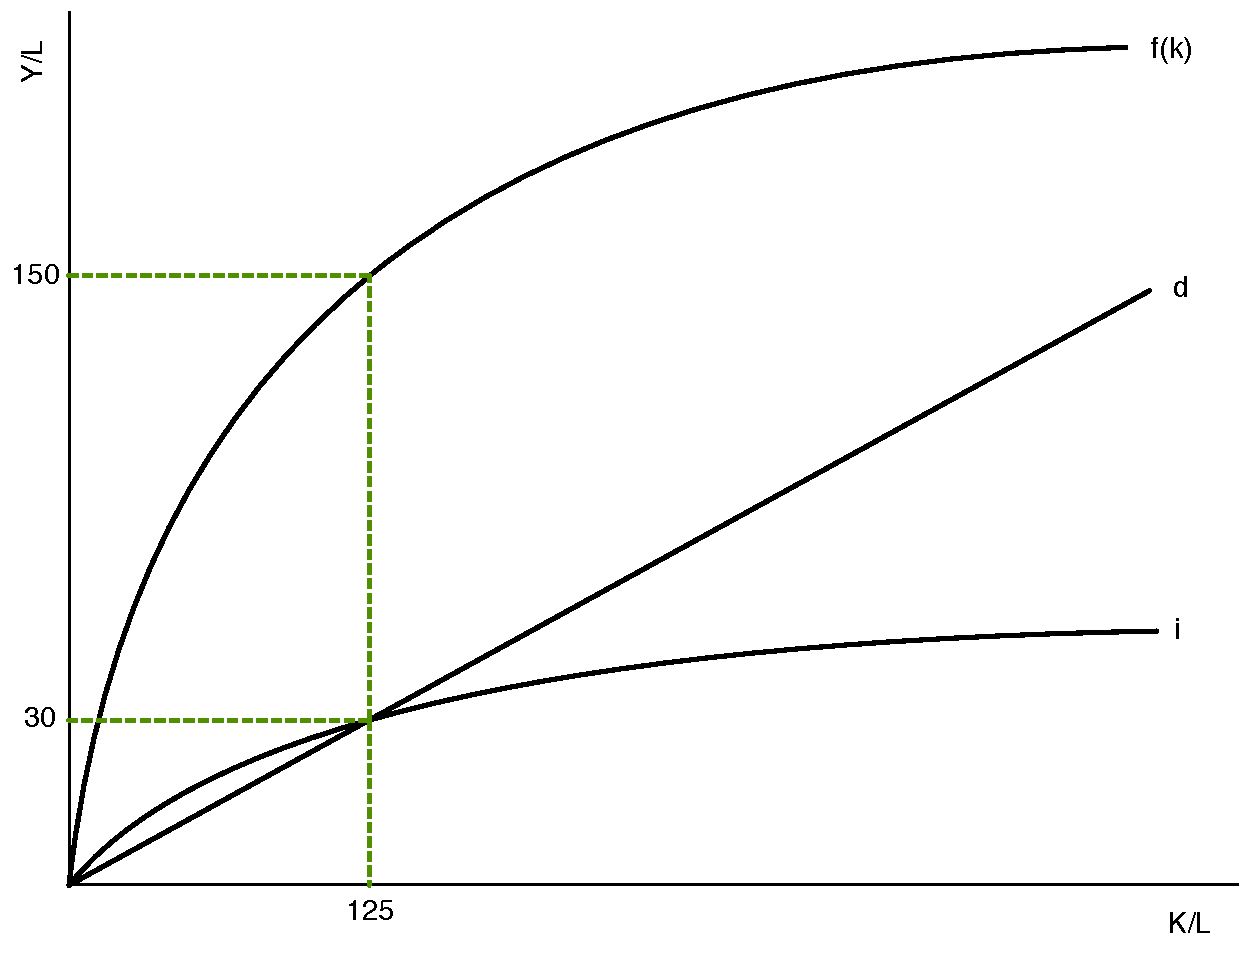
\includegraphics[scale=.35]{Final_MC22.pdf}
	\caption{Production, Investment, and Depreciation}
	\label{MC22}
\end{figure}

Country $X$ currently has $k^0_x$ units of capital and a negative rate of output growth, while country $Y$ currently has $k^0_y$ units of capital and a positive rate of output growth. If $k^*_x$ and $k_y^*$ denote the steady-state levels of capital in country $X$ and $Y$, respectively, which of the following statements is true?

\begin{choices}
	\choice $k^0_x < 125$ and $k^0_y > 125$
	\choice $k^*_x < 125$ and $k^*_y > 125$
	\choice $k^*_x > 125$ and $k^*_y < 125$
	\CorrectChoice $k^0_x > 125$ and $k^0_y < 125$
\end{choices}

\question Suppose a country is currently at its steady state. All else equal, if the country's depreciation rate permanently \underline{increases}, how many of the statements must be TRUE?


\begin{enumerate}[i.]
	\item The new steady state consumption level will be less than the old steady state consumption level.
	\item The new steady state investment level will be less than the old steady state investment level.
	\item The new steady state level of capital will be less than the old steady state level of capital,
	\item The new steady state level of output will be less than the old steady state level of output.
\end{enumerate}

\begin{choices}
	\choice 0 
	\choice 1
	\choice 2 
	\choice 3
	\CorrectChoice 4
\end{choices}

\newpage


\question Refer to Table \ref{tab3}. 

\begin{table}[H]
	\centering
	\caption{Production in Utopia}
	\label{tab3}
	\begin{tabular}{c|c|c}        
		
		$k$ & $y$ & $MP_k$ \\
		\hline
		1000 & 100 & --- \\
		1001 & $x$ & $z$ \\
		1002 & $y$ & 5 \\
		
	\end{tabular}
\end{table}

Under the assumptions of production functions in the Solow model, which of the following holds true?

\begin{choices}
	\CorrectChoice $x<y$ and $z>5$
	\choice $x>y$ and $z>5$
	\choice $x<y$ and $z<5$
	\choice $x>y$ and $z<5$
	\choice Impossible to know without more information.
\end{choices}


\uplevel{\subsection*{Savings \& Investment}}

	
\question A company is planning to finance the construction of a new factory, but has limited funds. In order to procure the necessary funds, the company is likely to 

\begin{choices}
	\choice demand loanable funds by buying bonds.
	\choice supply loanable funds by selling bonds.
	\CorrectChoice demand loanable funds by selling bonds.
	\choice supply loanable funds by buying bonds.
\end{choices}

\question A closed economy has private savings equal to \$500 billion and public savings of $-\$20$ billion. If consumption in the economy is \$400 billion and taxes equal \$50 billion, then government spending is \blank billion and total spending (i.e., GDP) in the economy is \blank billion.

\begin{choices}
	\CorrectChoice \$70; \$950
	\choice \$50; \$950
	\choice \$70; \$900
	\choice \$30; \$600
\end{choices}

\newpage

\question You buy a bond today that promises to pay \$50 in one year, \$50 in two years, and \$1,050 in three years. If the market interest rate is 6\% and remains so for the next three years, which of the following represents the price of the bond if you decide to sell it in one year after receiving the first \$50 payment?

\begin{choices}
	\choice $P = \frac{\$50}{(1.06)} + \frac{\$50}{(1.06)^2} + \frac{\$1,050}{(1.06)^3}$
	\CorrectChoice $P = \frac{\$50}{(1.06)} + \frac{\$1,050}{(1.06)^2}$
	\choice $P = \$50 + \frac{\$50}{(1.06)} + \frac{\$1,050}{(1.06)^2}$
	\choice $P = \$50 + \frac{\$1,050}{(1.06)}$
	\choice None of the above.
\end{choices}



\question In the presence of a savings tax credit, how many of the following are FALSE?

\begin{enumerate}[(i)]
	\item The real interest rate will increase.
	\item The quantity of investment will decrease.
	\item The quantity of savings will increase.
\end{enumerate}

\begin{choices}
	\CorrectChoice 2
	\choice 0
	\choice 1
	\choice 3
\end{choices}



\question Suppose you currently hold a bond that promises to pay \$100 in a year, \$100 in two years, and \$1,100 in three years. If you wish to sell the bond today in order to buy a new bicycle, which of the following market interest rates would allow you to sell the bond for the highest price?
\begin{choices}
	\CorrectChoice 5\%
	\choice 7\%
	\choice 10\%
	\choice 8\%
\end{choices}

	

\uplevel{\subsection*{Unemployment}}



\question Jack loses his job working as a consultant and decides to take time off to explore Europe. Jill has been looking for work for some time, but gave up looking for a job 2 months ago. Given this, Jack's actions will \blank the unemployment rate while Jill's will \blank the unemployment rate.

\begin{choices}
	\choice increase; increase
	\choice decrease; increase
	\choice	decrease; decrease
	\CorrectChoice increase; decrease
	\choice None of the above
\end{choices}


\question How many of the following will lead to the unemployment rate not being a good reflection of economic conditions?

\begin{enumerate}[i.]
	\item Woody leaves his job at UNC and starts his own toy shop business.
	\item Morgan wishes to have a job, but stopped looking for work after being discouraged by few call backs.
	\item Jonathan isn't actively looking for work, but claims to do so in order to receive unemployment benefits.
	\item Allen is fired from his job at McDonald's and immediately begins looking for work at other fast food joints.
\end{enumerate}

\begin{choices}
	\choice 0
	\choice 1
	\CorrectChoice 2
	\choice 3
	\choice 4
\end{choices}

	
\question John Doe looked for a new job for two months when he and his family moved to South Florida, but stopped looking for work six weeks ago because his wife landed a prominent position at the University of Miami. As of right now, John is considered \blank by the BLS.

\begin{choices}
	\choice frictionally unemployed
	\choice structurally unemployed 
	\CorrectChoice not in the labor force
	\choice cyclically unemployed
\end{choices}



\question Natalie just graduated from college. In order to devote all her efforts towards her education, she didn't hold a job while in school. Now, she is going to cruise around the country on her motorcycle for awhile before she starts looking for work. As a result, the unemployment rate

\begin{choices}
	\choice increases, and the labor-force participation rate increases.
	\CorrectChoice is unaffected, and the labor-force participation rate is unaffected.
	\choice increases, and the labor-force participation rate decreases. 
	\choice increases, and the labor-force participation rate is unaffected.
\end{choices}


\question Which of the following represents an example of structural unemployment?

\begin{choices}
	\choice Tina is currently looking for work as a Barista. She only started looking for work a few weeks ago, but it seems that most coffee shops are still recovering from an economic downturn and are hesitant to hire.
	\choice Jameson just moved to the City of Brotherly Love to find work as an accountant. It is taking him some time to polish his resume, send out applications, and receive call backs from interested firms.
	\choice The city council of Ski Mountain Resort observes that unemployment in the region increases during the summer months.
	\CorrectChoice Tommy worked at a factory, but was laid off recently because a machine could perform his job more efficiently.
\end{choices}

\uplevel{\subsection*{The Monetary System}}

\question Suppose the Fed sets the minimum reserve ratio at 25\%. If banks choose to hold 28\% of deposits as reserves and the Fed increases the money supply by \$5 million, then the maximum amount the money supply could potentially increase is


\begin{choices}
	\CorrectChoice less than \$18 million.
	\choice exactly \$20 million.
	\choice more than \$18 million but less than \$20 million.
	\choice more than \$20 million.
\end{choices}
	
	
\question Suppose an economy contains 2,000 \$1 bills. If people initially deposit half their currency as demand deposits while banks maintain 100\% reserves, the quantity of money would be \blank. If, however, people initially deposit all their currency as demand deposits while banks maintain 100\% reserves, the quantity of money is \blank.

\begin{choices}
	\CorrectChoice \$2,000; \$2,000
	\choice \$2,000; \$1,000
	\choice \$1,000; \$1,000
	\choice \$1,000; \$2,000
\end{choices}



\question Jonathan takes \$500 of currency from her wallet and deposits it in a checking account. If the bank adds the entire \$500 to reserves, the money supply \underline{\hspace{3cm}}, but if the bank lends out some of the \$500, the money supply \underline{\hspace{3cm}}.


\begin{choices}
	\choice increases; increases even more
	\choice increases; increases by less
	\CorrectChoice is unchanged; increases
	\choice decreases; decreases by less
\end{choices}

\question Which of the following policy combinations would consistently work to increase the money supply?

\begin{choices}
	\CorrectChoice Buy government bonds, decrease reserve requirements, and decrease the discount rate.
	\choice Sell government bonds, decrease reserve requirements, and decrease the discount rate.
	\choice Sell government bonds, increase reserve requirements, and increase the discount rate.
	\choice Buy government bonds, decrease reserve requirements, and increase the discount rate.
\end{choices}


\newpage

\uplevel{\subsection*{Money Growth \& Inflation}}



\question Unexpected deflation will

\begin{choices}
	\choice lower the real value of debts and redistribute wealth from lenders to borrowers.
	\CorrectChoice raise the real value of debts and redistribute wealth from borrowers to lenders.
	\choice lower the real value of debts and redistribute wealth from borrowers to lenders.
	\choice raise the real value of debts and redistribute wealth from lenders to borrowers.
\end{choices}

\question Consider Figure \ref{MC8}, which shows the market for money in Portlandia. $P$ is the overall price level in the economy.

\begin{figure}[H]
	\centering
	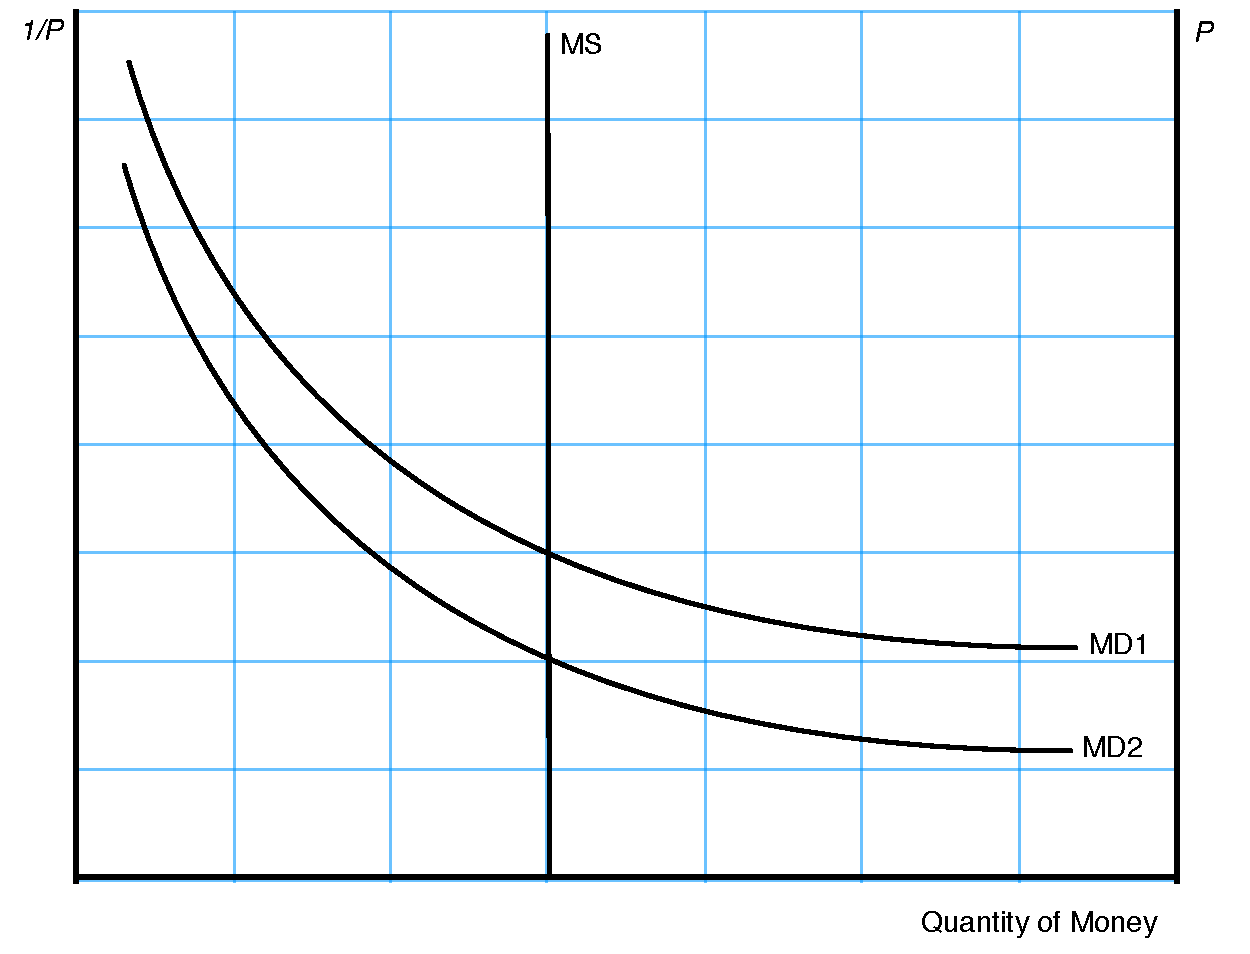
\includegraphics[scale=.40]{Final_MC8.pdf}
	\caption{The Money Market}
	\label{MC8}
\end{figure}

If the price level in the economy increased as a result of a money demand shift, then it must be that the money demand curve

\begin{choices}
	\choice shifted from MD1 to MD2 and the value of money increased.
	\CorrectChoice shifted from MD1 to MD2 and the value of money decreased.
	\choice shifted from MD2 to MD1 and the value of money decreased.
	\choice shifted from MD2 to MD1 and the value of money increased.
\end{choices}


\question You decide to put \$500 dollars into a savings account advertising 2\% annual interest. After a year, you withdraw your money and have to pay a tax of 20\% on your interest earnings. If inflation over the year was 1.75\%, then your after-tax nominal interest rate was \blank and your purchasing power \blank.

\begin{choices}
	\choice .35\%; increased
	\choice .6\%; decreased
	\CorrectChoice 1.6\%; decreased
	\choice .35\%; decreased
	\choice 1.6\%; increased
\end{choices}

\question Suppose you lend your roommate \$100 for one year at 12\% nominal interest. You both expect the real interest rate on the loan to be 9\%. If at the end of the loan wealth was transferred from your roommate to you, then actual inflation over the course of the year could have been

\begin{choices}
	\choice $7\%$.
	\choice $9\%$.
	\choice $14\%$.
	\CorrectChoice $0\%$.
	\choice Either (a) or (d).
\end{choices}

	\question Which of the following is NOT a cost of inflation?

\begin{choices}
	\choice Shoeleather costs
	\choice Tax distortions
	\choice Arbitrary redistribution of wealth
	\choice Menu costs
	\CorrectChoice All of the above are costs of inflation.
\end{choices}



\question The quantity theory of money concludes that an increase in the money supply causes

\begin{choices}
	\CorrectChoice a proportional increase in prices.
	\choice a proportional increase in velocity.
	\choice a proportional increase in real output.
	\choice a proportional decrease in velocity.
	\choice a proportional decrease in prices.
\end{choices}


\uplevel{\subsection*{Aggregate Demand \& Supply}}


\question Which of the following is an example of a negative real shock?

\begin{choices}
	\choice Consumers become pessimistic about the economy and spend less.
	\choice The Federal Reserve is concerned about inflation and decreases the money supply.
	\choice The government increases taxes on consumers.
	\CorrectChoice A hurricane destroys numerous factories along the shoreline.
	\choice All of the above. 
\end{choices}


\question Assume an economy currently has real GDP growth of 4\%. If spending growth along the current $AD$ curve is 4\%, then inflation must be \blank. Additionally, if the Federal Reserve decides to increase the discount rate then the aggregate demand curve will \blank.

\begin{choices}
	\choice 8\%; shift left
	\choice 0\%; shift right
	\CorrectChoice 0\%; shift left
	\choice 8\%; shift right
	\choice None of the above.
\end{choices}

\newpage

\question Refer to Figure \ref{fig2}.

\begin{figure}[H]
	\centering
	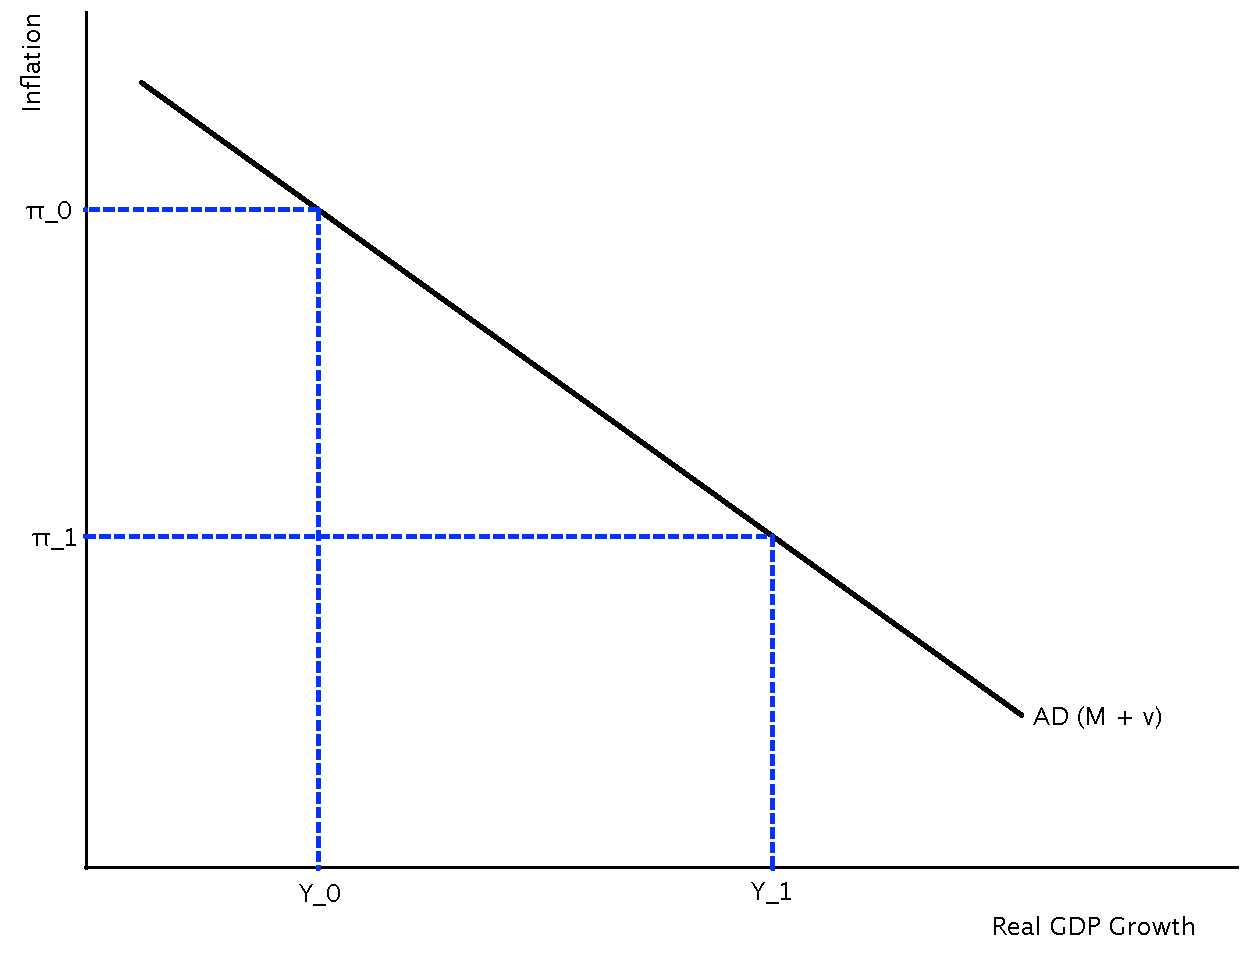
\includegraphics[scale=.40]{plot95.pdf}
	\caption{Aggregate Demand Curve}
	\label{fig2}
\end{figure}

Which of the following statements is correct?

\begin{choices}
	\choice $\pi_0 + \pi_1 = \vec{Y_0} + \vec{Y_1}$.
	\choice $\pi_0 + \vec{Y_1} = \pi_1 + \vec{Y_0}$.
	\choice $\pi_0 + \vec{Y_1} = \vec{M} + \vec{v}$.
	\choice $\pi_1 + \vec{Y_0} = \vec{M} + \vec{v}$.
	\CorrectChoice None of the above.
\end{choices}



\uplevel{Refer to Figure \ref{fig5} for questions \ref{qblah} - \ref{qblah2}.}

\begin{figure}[H]
	\centering
	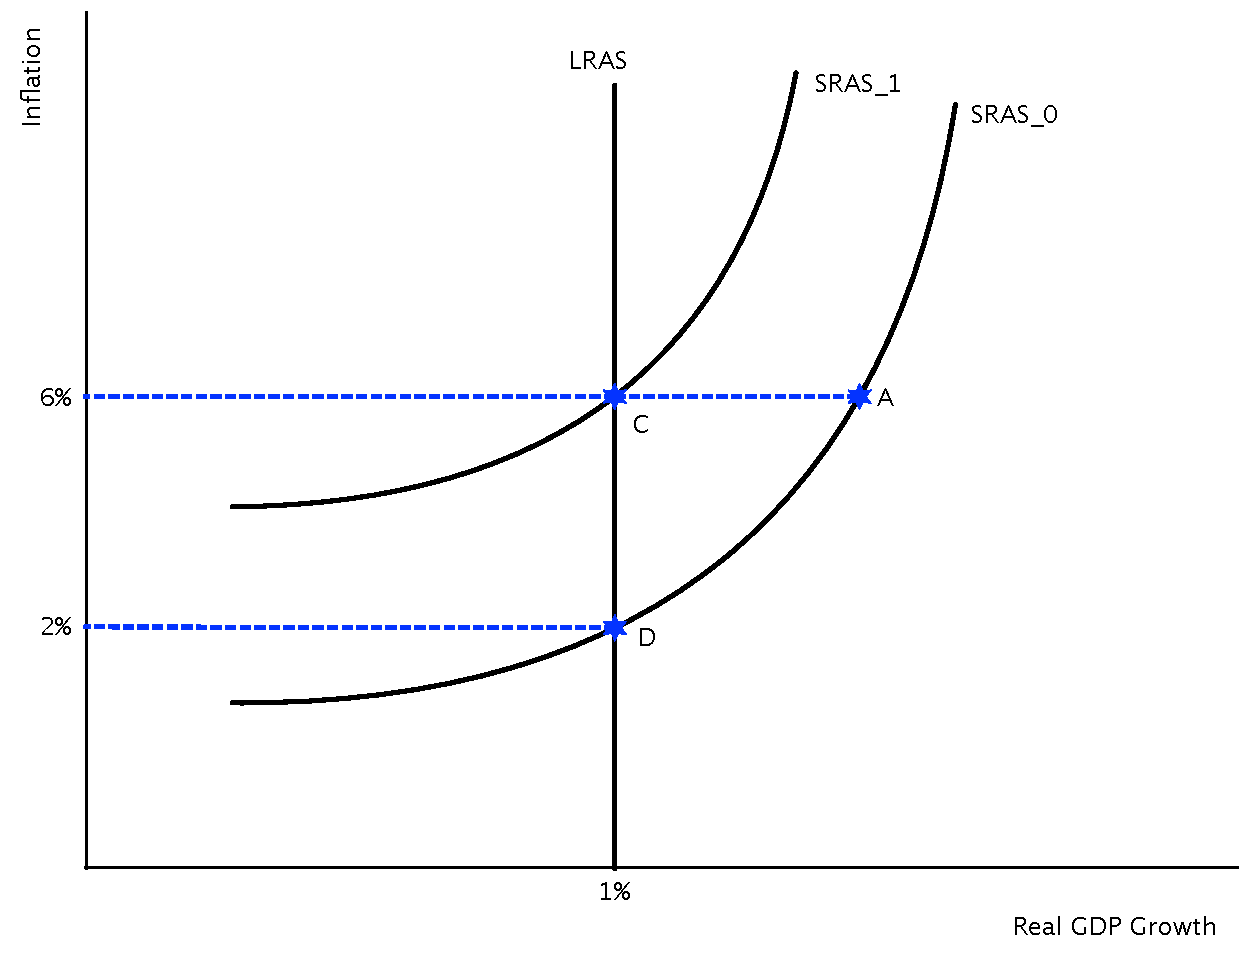
\includegraphics[scale=.40]{final_32.pdf}
	\caption{SRAS and LRAS}
	\label{fig5}
\end{figure}



\newpage

\question \label{qblah} Expected inflation at point $A$ is \blank, which is \blank actual inflation.

\begin{choices}
	\choice 2\%; greater than
	\CorrectChoice 2\%; less than
	\choice 6\%; equal to
	\choice 6\%; greater than
\end{choices}

\question At point $D$, expected inflation is 

\begin{choices}
	\choice less than expected inflation at point $A$.
	\choice more than expected inflation at point $A$.
	\choice more than expected inflation at point $C$.
	\CorrectChoice less than expected inflation at point $C$.
	\choice unknown.
\end{choices}

\question \label{qblah2} At point $A$, real GDP growth is

\begin{choices}
	\CorrectChoice greater than 1\%.
	\choice greater than 2\%.
	\choice equal to 1\%.
	\choice less than 1\%
	\choice unknown.
\end{choices}

\uplevel{\subsection*{Monetary \& Fiscal Policy}}

\question If the Federal Reserve wished to enact \underline{contractionary} monetary policy, how many of the following policies could be enacted to achieve their goal?

\begin{enumerate}[i.]
	\item Increase the discount rate
	\item Increase taxes
	\item Open market purchases of government bonds
\end{enumerate}

\begin{choices}
	\choice 0
	\CorrectChoice 1
	\choice 2
	\choice 3
\end{choices}

\question Suppose spending growth in the economy is currently 1\%. If the Federal government increases their spending by 4\% and spending growth in the economy is now 3\%, we can say that

\begin{choices}
	\choice The government enacted contractionary fiscal policy
	\CorrectChoice The multiplier effect was less than the crowding out effect
	\choice The multiplier effect was greater than the crowding out effect
	\choice The aggregate demand curve shifted to the left as a result of this policy.
\end{choices} 

\uplevel{Consider Figure \ref{mc40} for questions \ref{MC39} - \ref{MC40}.}

\begin{figure}[H]
	\centering
	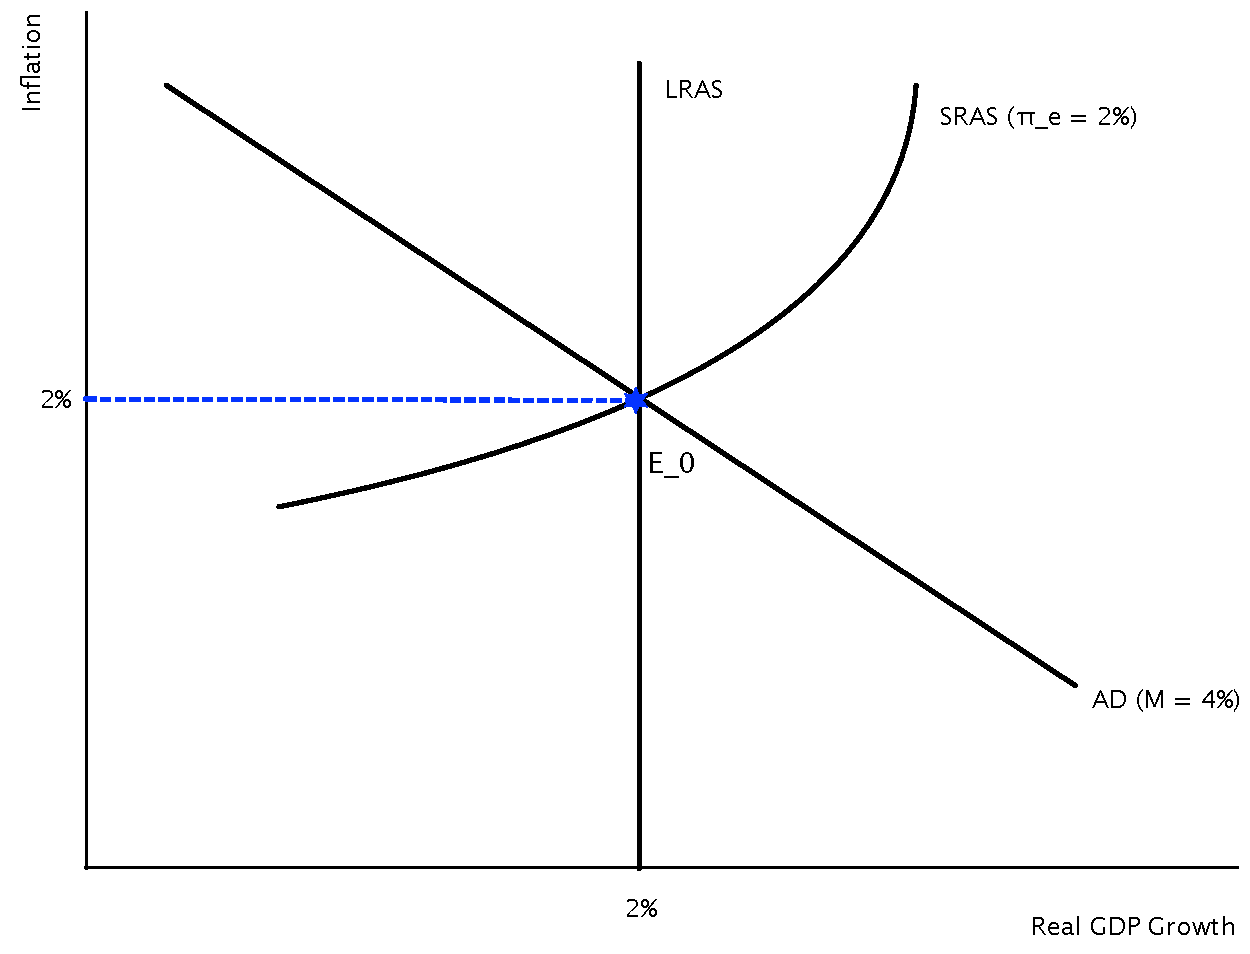
\includegraphics[scale=.40]{hw6_plot1.pdf}
	\caption{SRAS and LRAS}
	\label{mc40}
\end{figure}

\question \label{MC39} The Economy is currently operating at point $E_0$ and money growth is 3\%. Now, suppose that spending growth permanently decreases by 5\% due to a decrease in consumption spending. If this causes real GDP in the short-run to fall to $-2\%$, the inflation in the short-run will be 

\begin{choices}
	\CorrectChoice 1\%
	\choice 0\%
	\choice 2\%
	\choice 6\%
	\choice 4\%
\end{choices}  

\question \label{MC40} If the economy was still at its short-run equilibrium and the Federal Reserve wished to return the economy to its original long-run point $E_0$, then they would need to

\begin{choices}
	\choice increase money growth to 5\%.
	\choice increase money growth to 10\%
	\CorrectChoice increase money growth to 8\%.
	\choice increase money growth to 6\%.
\end{choices}

\uplevel{\subsection*{Introduction to Economics}}

\question A rational individual will partake in some action as long as

\begin{choices}
	\choice the total benefit exceeds the total cost.
	\choice the marginal benefit exceeds the opportunity cost.
	\CorrectChoice the marginal benefit exceeds the marginal cost.
	\choice the marginal benefit is positive.
\end{choices}

\newpage

\question The opportunity cost of a choice is defined as 

\begin{choices}
	\CorrectChoice the total value of the next best alternative.
	\choice the total value of all other alternatives.
	\choice the out-of-pocket costs of the next best alternative.
	\choice the total value of the selected choice.
\end{choices}


\uplevel{\subsection*{The Gains from Trade}}

\question Suppose Kenya and Sri Lanka have the opportunity costs of producing limes and oranges outlined in  Table \ref{blah}.

\begin{table}[H]
	\caption{Opportunity cost of one:}
	\centering
	\begin{tabular}{ c|c|c} 
		
		& Lime & Orange \\
		\hline
		Kenya & 1/2 & $x$  \\
		Sri Lanka & $y$  & 8  \\
	\end{tabular}
	\label{blah}
\end{table}.

Given this information, we can say that

\begin{choices}
	\choice Kenya has the comparative advantage in producing limes and Sri Lanka has the comparative advantage in producing oranges.
	\choice Kenya has the absolute advantage in producing oranges and Sri Lanka has the absolute advantage in producing limes.
	\choice Kenya has the absolute advantage in producing limes and Sri Lanka has the absolute advantage in producing oranges.
	\CorrectChoice Kenya has the comparative advantage in producing oranges and Sri Lanka has the comparative advantage in producing limes.
\end{choices}


\question The gains from trade are the result of two partners trading based off their 

\begin{choices}
	\CorrectChoice comparative advantage.
	\choice absolute advantage.
	\choice total productivity.
	\choice technological advantage.
\end{choices}

\uplevel{\subsection*{Supply and Demand}}

\uplevel{Consider each of the following scenarios for questions \ref{qq1} - \ref{qq2}.}

\begin{enumerate}[i.]
	\item The university book store has a fire sale on new textbooks at the end of the semester.
	\item The price of used textbooks falls.
	\item The expected future price of new textbooks increases.
	\item A hurricane destroys many of the trees used to create pulp for paper.
\end{enumerate}

\newpage

\question \label{qq1} How many of the statements would shift the demand curve in the market for new textbooks?

\begin{choices}
	\choice 1
	\choice 0
	\choice 3
	\CorrectChoice 2
	\choice 4
\end{choices}

\question \label{qq2} How many of the statements would increase the current price of new textbooks?

\begin{choices}
	\choice 1
	\CorrectChoice 2
	\choice 0
	\choice 3
	\choice 4
\end{choices}

\question Table \ref{MC17} shows the quantity supplied and demanded at certain prices.


\begin{table}[H]
	\caption{Prices and Quantities}
	\centering
	\begin{tabular}{  c | c | c} 
		
		Price & $Q_d$ & $Q_s$ \\
		\hline
		\$10 & 50 & 30 \\
		\$12 & 45 & 35 \\
		\$14 & 40 & 40 \\
		\$16 & 35 & 45 \\
		\$18 & 30 & 50 \\
	\end{tabular}
	\label{MC17}
\end{table}

If there is currently a surplus of 15 units, then the price in the market must be

\begin{choices}
	\CorrectChoice greater than \$16, but less than \$18.
	\choice less than \$14.
	\choice greater than \$14, but less than \$16.
	\choice greater than \$18.
\end{choices}


\uplevel{\subsection*{Government Policy}}

\question A price ceiling is only binding if it is set

\begin{choices}
	\choice above the equilibrium market price.
	\choice equal to the equilibrium market price.
	\CorrectChoice below the equilibrium market price.
	\choice either above or below the equilibrium market price - price ceilings are always binding.
\end{choices} 

\newpage

\question Suppose the government is deciding on between imposing a tax on cigarettes or on luxury, P-Diddy style house boats. If their goal is to minimize the deadweight losses from the tax, the government should impose the tax on

\begin{choices}
	\choice either market - the deadweight loss will be the same.
	\choice the market for house boats.
	\CorrectChoice the market for cigarettes.
	\choice neither market - the deadweight loss will necessarily exceed the tax revenues in both cases.
\end{choices}

\question A binding minimum wage in the market for labor is an example of a \blank and will create a \blank.

\begin{choices}
	\choice price ceiling; shortage of labor
	\choice price floor; shortage of labor
	\CorrectChoice price floor; surplus of labor
	\choice price ceiling; surplus of labor
\end{choices}




\question A subsidy provided in a market with no externalities will create a deadweight loss because 

\begin{choices}
	\choice it will reduce the number of transactions taking place, leading to unrealized gains from trade.
	\CorrectChoice it will increase the number transactions taking place, leading to inefficient transactions.
	\choice it will decrease both consumer and producer surplus.
	\choice the increase in consumer and producer surplus is greater than the cost of the subsidy.
\end{choices}


\uplevel{\subsection*{The Public Sector}}

\question In the presence of a negative externality, the government can maximize efficiency by

\begin{choices}
	\choice imposing a subsidy equal to the size of the external cost.
	\CorrectChoice imposing a tax equal to the size of the external cost.
	\choice imposing a tax smaller than the size of the external cost.
	\choice imposing a tax greater than the size of the external cost.
	\choice None of the above maximize efficiency.
\end{choices}

\newpage
	
\question Consider Figure \ref{MC25}. 

\begin{figure}[H]
	\centering
	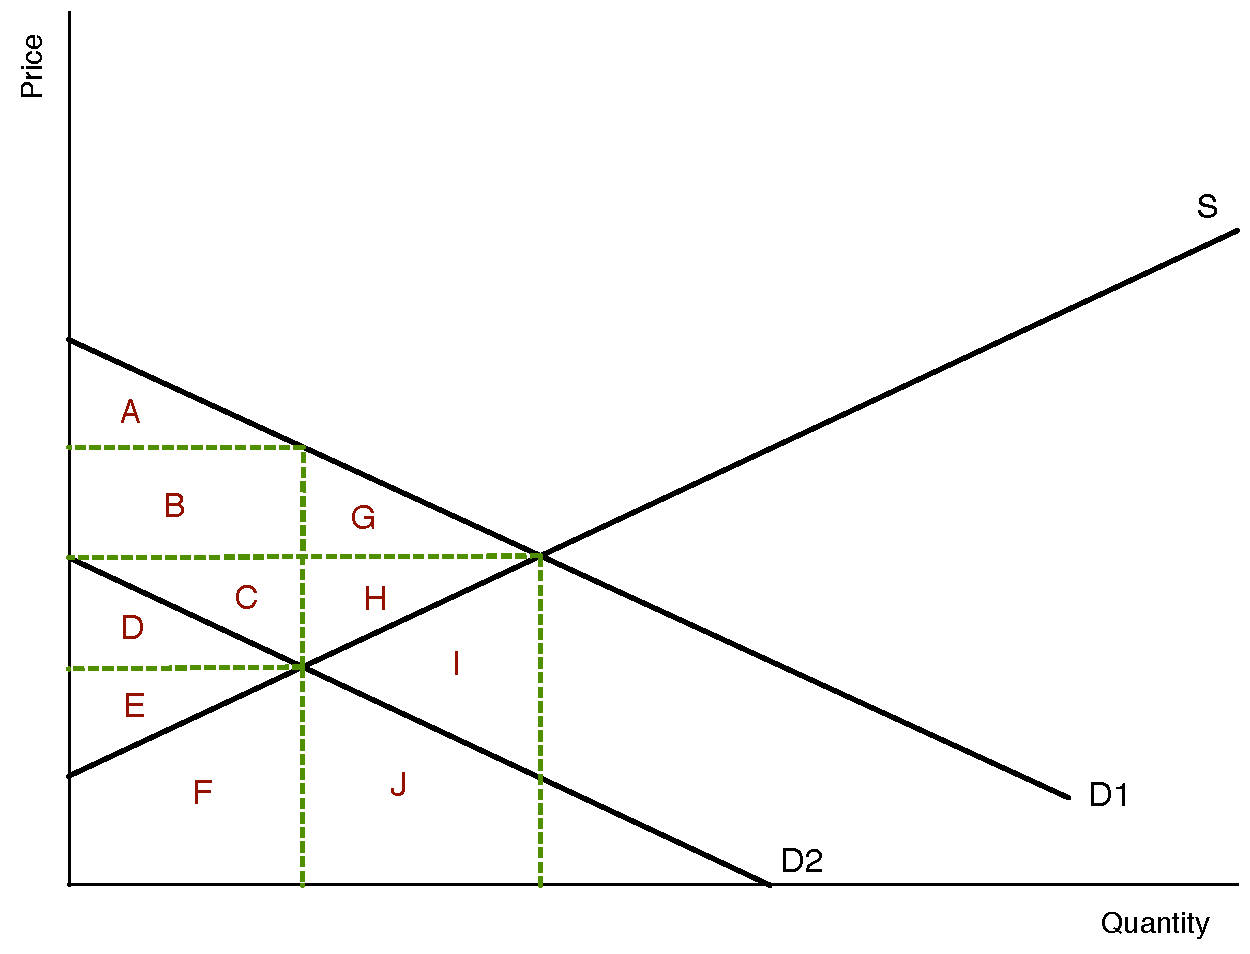
\includegraphics[scale=.40]{Exam1_MC25.pdf}
	\caption{Market for Fanta}
	\label{MC25}
\end{figure}

Suppose that the curve labeled D1 represents the social value curve in this market. In the absence of government intervention, the deadweight loss in the market is represented by area

\begin{choices}
	\CorrectChoice G + H
	\choice G + H + I
	\choice A + B + C
	\choice D + E
\end{choices}

\uplevel{\subsection*{Industrial Organization}}

\question Which of the following regarding a firm's production function (assuming labor is their only input) is TRUE?

\begin{choices}
	\CorrectChoice Eventually, the marginal product of labor will be decreasing.
	\choice The marginal product of labor decreases initially, but continuously increases after some amount of labor.
	\choice The marginal product of labor is always constant regardless of how much labor is employed.  
	\choice The marginal product of labor is always increasing regardless of how much labor is employed.  
\end{choices}


\newpage


\question Which of the following is true regarding the relationship between the \underline{price} charged by a monopoly, an oligopoly acting as a cartel, an oligopoly that is not cooperative, and a perfectly competitive firm?

\begin{choices}
	\choice monopoly > cartel > non-cooperative oligopoly > perfectly competitive firm
	\choice  monopoly > cartel > non-cooperative oligopoly = perfectly competitive firm
	\choice  monopoly = non-cooperative oligopoly > cartel > perfectly competitive firm
	\CorrectChoice  monopoly = cartel > non-cooperative oligopoly > perfectly competitive firm
\end{choices}


\question Consider the game matrix below.

\renewcommand{\gamestretch}{1.5}
\sgcolsep=25pt
\begin{figure}[H]\hspace*{\fill}%
	\begin{game}{3}{3}[Noah][Isabella] 
		&  Run & Walk & Crawl \\
		Run & 4, 1 & 4, 4 & 1, 2 \\
		Walk & 3, 4 & 1, 3 & 3, 2 \\
		Crawl & 2, 4 & 2, 3 & 4, 6 \\
	\end{game} 
	\hspace*{\fill}%
\end{figure}

How many Nash Equilibria does this game have?

\begin{choices}
	\CorrectChoice 2
	\choice 3
	\choice 1
	\choice 4 or more
	\choice 0
\end{choices}



\uplevel{\subsection*{GDP and the CPI}}


\question Table \ref{MC23} shows the prices and quantities produced of the only two goods in Uzbeki-beki-beki-Stan-Stan, grapes and olives, for the years 2000 and 2001. Assume 2000 is the base year.

\begin{table}[H]
	\caption{Grapes and Olives in UZN}
	\centering
	\begin{tabular}{c|c|c|c|c}
		Year & Grapes Produced & Price of Grapes & Olives Produced & Price of Olives \\
		\hline
		2000 & 20 & \$2.10 & 25 & \$4.10\\
		2001 & 18 & $x$ & 15 & $y$ \\
	\end{tabular} 
	\label{MC23}
\end{table}

In 2001, the value of real GPD 

\begin{choices}
	\choice cannot be determined from this information.
	\choice is greater than real GDP in 2000.
	\choice is equal to real GDP in 2000.
	\CorrectChoice is less than real GDP in 2000.
\end{choices}


\newpage


\question How many of the following transactions would affect the investment component of US GDP? Assume all of the transactions occur within the United States.

\begin{enumerate}[(i)]
	\item Tina's Housekeeping Company purchases a new laptop that was manufactured in China.
	\item Jane purchases a new bookshelf from Macy's.
	\item Your parents buy government bonds.
	\item A newly-wed couple buys a newly constructed home.
\end{enumerate}

\begin{choices}
	\choice 1
	\CorrectChoice 2
	\choice 0
	\choice 3
	\choice 4
\end{choices}	

\question Suppose the nominal yearly earnings of minimum wage workers was \$35,000 in both 2000 and 2010. If the purchasing power of minimum wage workers increased, it must be that

\begin{choices}
	\choice the CPI in 2000 is lower than the CPI in 2010.
	\CorrectChoice the CPI in 2010 is lower than the CPI in 2000.
	\choice the CPI in 2000 is the same as the CPI in 2010.
	\choice any of the above could be true.
\end{choices}



\question Table \ref{blahan} shows the prices and quantities consumed of the only two goods in Uzbeki-beki-beki-Stan-Stan, grapes and olives, for the years 2010 and 2011. Assume that the typical basket of grapes and olives was determined by the quantity of each consumed in 2010.

\begin{table}[H]
	\caption{Grapes and Olives in UZN}
	\centering
	\begin{tabular}{c|c|c|c|c}
		Year & Grapes Consumed & Price of Grapes & Olives Consumed & Price of Olives \\
		\hline
		2010 & 20 & \$2.10 & 25 & \$4.10\\
		2011 & $x$ & \$2.15 & $y$ & \$4.25 \\
	\end{tabular} 
	\label{blahan}
\end{table}

In 2011, the value of the Consumer Price Index (CPI) 

\begin{choices}
	\CorrectChoice is greater than the CPI in 2010.
	\choice is equal to the CPI in 2010.
	\choice is less than the CPI in 2010.
	\choice cannot be determined from this information.
\end{choices}


\end{questions}	



\end{document}